\chapter{\texorpdfstring{\acrshort{knn}}{kNN} queries in the snapshot model}\label{section:knn-snapshot}
\thispagestyle{myheadings}

	In this chapter I analyze secure \acrshort{knn} queries in the snapshot adversary model.
	I study the effect of protecting the records with a type of property-preserving encryption on quality of search and efficiency of certain attacks.
	Specifically, I examine theoretically and practically how accuracy of both \acrshort{knn} search and \acrshort{ml}-based inversion attack degrade with added security.

	\section{Introduction}

		Nearest-neighbor search is a type of optimization problem that, given a set of objects and a distance metric, requires finding the object closest to a given point according to the distance metric.
		A \acrfull{knn} search is a subtype of a general nearest-neighbor problem where $k$ closest objects are requested.
		Applications that use \acrshort{knn} search only need to define the objects and the metric.
		For example, a street map application would define the 2D coordinates of the buildings as objects and Euclidean distance as a metric, then the query could be ``give 5 restaurants closest to the current user position''.
		A document search application would define the keyword vector for a document as an object and an inner product distance as a metric, then the query could be ``give 3 documents most similar to the given text'' (similar applications may search images, videos and sounds).

		In this chapter we propose a method and an analysis of running secure \acrshort{knn} queries in outsourced database model.
		We model our application as a generic document similarity search, where the server stores the embeddings of the documents and returns $k$ closest records to the query embedding.
		We propose to apply a type of property-preserving encryption over the embeddings on the server while retaining its ability to do nearest-neighbor search.
		Finally, we simulate an attack against the records --- an \acrshort{ml}-based inversion attack that aims to recover the set of words of a document from its embedding.
		Our goal is to observe and study the correlation of the security parameter with search accuracy and attack efficiency.

		To summarize, our contributions in this work are as follows:
		\begin{itemize}
			\item
				We adapt and implement a \acrfull{dcpe} scheme from \cite{dcpe} to encrypt text embeddings.
				We analyze the practical aspects of \acrshort{dcpe} scheme's security (e.g., the effects of floating point representation) and benchmark the construction.

			\item
				We conduct a set of experiments to study the effect of security parameter on search accuracy.
				We use a fine-tuned \acrshort{bert} model\footnote{Provided by Hamed Zamani} to produce embeddings for the \acrshort{trec} 2020 collection.
				Given \acrshort{trec} validation set (i.e., ``correct answers'') we run the search for varying security levels and report a number of ranking quality measures.

			\item
				We adapt a recent \acrshort{ml}-based inversion attack by \textcite{embedding-attacks} against embeddings to our setting.
				The attack works by training an \acrshort{lstm} model on pairs of sentences and their embeddings.
				We run this attack for varying security levels, and training on both plaintext and encrypted records.

			\item
				Finally, we analyze the correlation results for search accuracy and attack efficiency and conclude on practicality of our method.
		\end{itemize}

		\subsection{Related Work}

			Work in this area is naturally split into two groups --- mechanisms and constructions that offer certain security guarantees for nearest-neighbor queries, and attacks against those constructions.

			A work immediately related to ours is QuickN by \textcite{quick-n}.
			QuickN offers an adaptation of nearest-neighbor search algorithm in conventional tree data structures (i.e., R-trees) to well-established \acrfull{ope} schemes.
			Unlike our solution that involves a novel property-preserving encryption scheme specifically designed for high-dimensional vectors, QuickN encrypts each vector dimension separately with \acrshort{ope}.
			\cite{quick-n} includes the experiments with attacks against their solution (attack by \textcite{leakage-abuse-grubs-2017}) and report high degree of protection against them.

			QuickN approach of applying \acrshort{ope} to an R-tree, however, has some disadvantages.
			First, an ideal stateless \acrshort{ope} has been shown inferior (\cite{ope-leakage}) to its counterpart, an \acrfull{ore} in which the comparison over ciphertexts is defined explicitly.\footnote{
				\cite{quick-n} uses mOPE \cite{ope-ideal-security-protocol} which is an interactive protocol and not a traditional lightweight stateless \acrshort{ope} like \cite{bclo-ope}.
				Since mOPE is an ideal (though stateful) \acrshort{ope}, \cite{quick-n} do not include \acrshort{ope} leakage in their security definition.
			}
			An \acrshort{ore}, in turn, can have a varying level of security, with the higher security level translating into lower comparison performance \cite{ore-benchmark-17}.
			In QuickN, an R-tree-based nearest-neighbor algorithm involves a very high number of comparisons, linear in data dimensionality.
			With the cost of comparison no longer negligible, the overhead of query over 2D or 3D is already high, saying nothing of 768-dimensional vectors that our work targets.
			Second, QuickN protocol is not single-round (i.e., it takes two roundtrips per query) and it returns a large number of false positive results even for a minimal $k$ (\num{4000} false positives for $10^6$ dataset and $k = 1$).

			\textcite{knn-aspe} offer a novel scheme, ASPE, that preserves a special type of scalar product.
			ASPE is then naturally integrated in existing \acrshort{knn} algorithms that rely on a scalar product.
			\cite{knn-aspe} is similar to ours in that we also apply a property-preserving encryption scheme to existing \acrshort{knn} algorithms.
			ASPE is different in that it preserves a scalar product while we preserve an $\text{L}_2$ distance comparison, and ASPE has been broken in \cite{secure-nn-revisited-break-aspe} (although an attack is a chosen plaintext attack, i.e., one cannot decrypt a random ciphertext).

			Other works either target different aspects of query security, like integrity and soundness of results \cite{knn-integrity-soundness,svknn}, or involve mechanisms other than property-preserving encryption \cite{seceqp,practical-approx-knn,knn-sharing-keys,knn-mult-data-owners,knn-over-encrypted,knn-paillier,knn-blind,knn-homomorphism,knn-strong-location-privacy,knn-no-anonymizers,knn-efficient,knn-new-casper}.

	\section{\texorpdfstring{\acrlong{dcpe}}{Distance Comparison Preserving Encryption}}

		A promising approach in secure \acrshort{knn} evaluation is using a property-preserving encryption scheme to allow the existing search algorithms to work with minimal alterations.
		ASPE scheme by \textcite{knn-aspe} is a step in this direction, but a scheme has been shown insecure under a type of chosen plaintext attack in \cite{secure-nn-revisited-break-aspe}.
		Using a common \acrshort{ope} scheme over vector values has been explored in \cite{quick-n}, but this approach incurs high overhead linear in dimensionality.
		We, therefore, need a different method --- a scheme that operates over high-dimensional vectors and preserves a property that is required to answer the nearest-neighbor queries.

		A classical nearest-neighbor search \cite{knn-wong,knn-cunningham} simply orders the objects according to their distances from the target.
		It is important to note that knowing the exact distance is not required, merely the knowledge of \emph{distance comparison} suffices (i.e., $x$ is closer to $y$ than $z$ is).
		An encryption scheme that preserves the distance comparison would satisfy the \acrshort{knn} search correctness, but not necessarily security or even practicality.
		First, a fully deterministic \acrfull{dcpe} would reveal at least the frequency of data points (i.e., how many times a point appears in the dataset).
		Second, even in the plaintext world the use of approximate nearest-neighbor search \cite{scalable-nn,approximate-nn-fixed-d} may be preferred due to the curse of dimensionality \cite{nn-meaningful,nn-curse-of-d} (exact distance is less important in higher dimensions).

		\subsection{\texorpdfstring{\acrshort{dcpe}}{DCPE} construction}

			A candidate \emph{approximate} \acrshort{dcpe} scheme that we adapt to our solution has been recently proposed by \textcite{dcpe}.
			The scheme provides the following guarantee on its ciphertexts
			\begin{multline*}
				\forall x, y, z \in \mathbb{X} : \algo{Dist}{x, y} < \algo{Dist}{x, z} - \beta \\
				\implies \algo{Dist}{f(x), f(y)} < \algo{Dist}{f(x), f(z)}
			\end{multline*}
			where $\mathbb{X} \subseteq \mathbb{R}^d$ is the set of $d$-dimensional vectors of real numbers, \algo{Dist} is the $\text{L}_2$ distance over elements in $\mathbb{X}$, and $\beta$ is the approximation term.
			Parameter $\beta$ partially defines the security of the encrypted set --- the larger $\beta$, the fewer distance comparisons are preserved, the less accurate the search and the reconstruction attacks would be.
			\textcite{dcpe} prove protection against membership inference attacks \cite{memebership-inference-attacks-knn} (whether an individual is in the database or not), and against the approximate frequency-finding attacks (how many times the element appears in the set, see \cite{leakage-abuse-grubs-2017} for \acrshort{ore} frequency attacks).
			As for the choice of $\beta$, \textcite{dcpe} prove that $\beta \approx \sqrt{\max N}$ would hide about half of the input bits, for $\max N$ being the maximum vector length in the dataset.

			% chktex-file 1
% chktex-file 8

\newlength{\dcpeAlgInterLength}
\setlength{\dcpeAlgInterLength}{0.18ex}

\begin{algorithm*}[ht!]

	\begin{pchstack}

		\procedure[linenumbering]{\algo{KeyGen}{\secparam, \mathbb{S}}}{
			s \sample \mathbb{S}		\\
			\key \sample \bin^\secpar	\\
			\pcreturn (s, \key)
		}

		\hspace{\dcpeAlgInterLength}

		\procedure[linenumbering]{\algo{Enc}{ (s, \key), \vec{m} }}{
			n \sample \bin^\secpar														\\
			\mathsf{coins}_n || \mathsf{coins}_u \gets \algo{\acrshort{prf}}{\key, n}	\\
			\vec{n} \sample \algo{Normal}{0, I_d; \mathsf{coins}_n}						\\
			u \sample \algo{Uniform}{0, 1; \mathsf{coins}_u}							\\
			x \gets \frac{s \beta}{4} \cdot \sqrt[d]{u}									\\
			\vec{\delta} \gets \frac{\vec{n}}{\|\vec{n}\|} \cdot x						\\
			\vec{c} \gets s \cdot \vec{m} + \vec{\delta}								\\
			\pcreturn \vec{c}
		}

		\hspace{\dcpeAlgInterLength}

		\procedure[linenumbering]{\algo{Dec}{ (s, \key), (\vec{c}, n) }}{
			\mathsf{coins}_n || \mathsf{coins}_u \gets \algo{\acrshort{prf}}{\key, n}	\\
			\vec{n} \sample \algo{Normal}{0, I_d; \mathsf{coins}_n}						\\
			u \sample \algo{Uniform}{0, 1; \mathsf{coins}_u}							\\
			x \gets \frac{s \beta}{4} \cdot \sqrt[d]{u}									\\
			\vec{\delta} \gets \frac{\vec{n}}{\|\vec{n}\|} \cdot x						\\
			\vec{m} \gets \frac{\vec{c} - \vec{\delta}}{s}								\\
			\pcreturn \vec{m}
		}

	\end{pchstack}

	\caption[\acrshort{dcpe} scheme]{
		\acrlong{dcpe} scheme, adapted from \cite[Algorithm 2]{dcpe}.
	}%
	\label{algorithm:dcpe}
\end{algorithm*}


			\textcite{dcpe} offer an instantiation of the $\beta$-\acrshort{dcpe} scheme (though not an implementation) that we have adapted to our needs and show on \cref{algorithm:dcpe}.

			The \algo{KeyGen} procedure generates a key \key{} and an amplification factor $s$.

			The \algo{Enc} procedure ``encrypts'' an object by moving it in space in a way that makes it hard to recover its original position and its distance-comparison respective to other encrypted points is preserved.
			The algorithm first constructs a hyperball of radius $\beta$, the approximation term, around the input point.
			The routine then samples a new point uniformly inside that hyperball.
			Finally, that new point is projected into the ciphertext point according to the amplification factor $s$.
			Note that for each encryption the scheme generates a fresh nonce $n$ and uses it along with the key \key{} to generate the coins for the samplers.
			That is, the point in the $\beta$-hyperball is deterministically set from the nonce (unique per point) and the key (one for all points), and the final ciphertext is scaled the same way for all points.
			The \algo{Dec} procedure makes the same steps in reverse correctly setting the point in the hyperball using the nonce and the key.
			See \cref{figure:dcpe} for a visual example of \acrshort{dcpe} encryption.

			\begin{figure}[!ht]
	\centering
	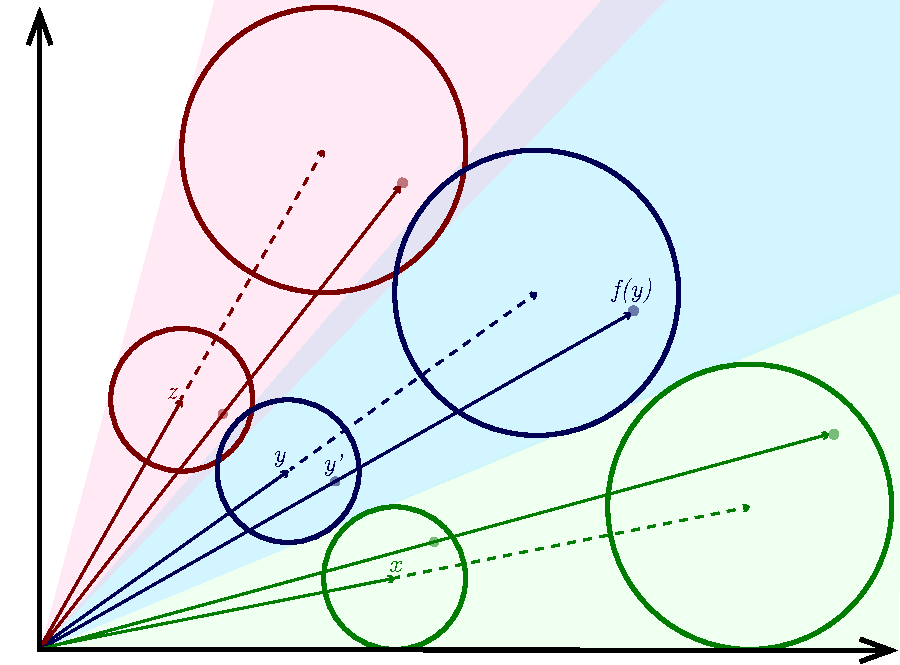
\includegraphics[width=1.0\textwidth]{dcpe}
	\caption[Schematic description of \acrshort{dcpe}]{
		Schematic description of encryption process of \acrshort{dcpe}, drawn to scale.
		In this diagram, there are two dimensions ($d = 2$), $\beta$ (the radius of a circle) is 2 units, and $s$ (the projection magnitude, the length from the origin to the larger circle over the length to the smaller one) is 2.
		The encrypted point is uniformly sampled inside a $\beta$-sphere, then projected $s$ times further from the origin.
		If two points are too close, their circles intersect, and their encryptions can be sampled in a way that breaks distance comparison.
		Intuitively, larger $\beta$ implies greater ciphertext space for a point and greater security.
	}\label{figure:dcpe}
\end{figure}


		\subsection{\texorpdfstring{\acrshort{dcpe}}{DCPE} security}

			The security of the scheme thus depends on
			\begin{enumerate*}[label={(\roman*)}]
				\item the maximum amount of amplification,
				\item the radius of the hyperball $\beta$, and
				\item the entropy of the samplers.
			\end{enumerate*}
			\textcite{dcpe} show that the amplification, $s$ parameter, affects one-wayness bounds \cite[Section 7.2]{dcpe}.
			Approximation term $\beta$ affects bit-security with $\beta \approx \sqrt{\max N}$ protecting about half of the bits.
			Finally, the key \key{} and nonce $n$ sizes, the security parameter \secparam{}, and the samplers used to generate normal multivariate and uniform samples affect the specific amount of entropy used to generate a point in the hyperball.

			As the construction operates on real numbers, an open question remains on how to avoid negative side-effects of floating point numbers bit representation.
			Unlike integers, floating point numbers are represented in memory in a way that their precision is different depending on their value, see the IEEE 754-2019 standard \cite{ieee-floating-point}. % chktex 8
			Simply put, the closer the value is to zero, the smaller the difference between two consecutive representable values is.
			For example, while the representable 32-bit IEEE 754 floating point numbers range from about $1.18 \cdot 10^{-38}$ to $3.4 \cdot 10^{38}$, there are only $2^{32} \approx 4 \cdot 10^9$, 4 billion representable numbers.
			This, along with the rounding errors, puts some limits on how large $s$ and $\beta$ can be.

		\subsection{\texorpdfstring{\acrshort{dcpe}}{DCPE} implementation and benchmarks}

			We offer the first implementation of \cite{dcpe} $\beta$-\acrshort{dcpe} for 32- and 64-bit IEEE 754 numbers in C++.\footnote{
				\url{https://github.com/private-knn/dcpe}
			}
			The code is documented, tested and benchmarked, see \cref{table:dcpe-benchmarks}.
			Observe that the difference in performance between encryption and decryption is predictably minimal, and the overhead of encryption grows slower-than-linearly with dimensionality.
.
			{
	\def\arraystretch{1.0}
	\begin{table}[!ht]
		\begin{tabular*}{\linewidth}{ !{\extracolsep\fill} l l c l } % chktex 26
			\toprule
				Operation						& Input size								& Dimensions $d$	& Wall-clock time			\\
			\midrule
				\algo{KeyGen}					& N/A										& N/A				& \SI{1.81}{\milli\second}	\\
			\midrule
				\multirow{6}{*}{\algo{Enc}}		& \multirow{3}{*}{32-bit (\texttt{float})}	& 1					& \SI{4.12}{\milli\second}	\\
												& 											& 100				& \SI{12.2}{\milli\second}	\\
												& 											& 768				& \SI{62.0}{\milli\second}	\\ \cline{2-4}
												& \multirow{3}{*}{64-bit (\texttt{double})}	& 1					& \SI{3.96}{\milli\second}	\\
												& 											& 100				& \SI{11.4}{\milli\second}	\\
												& 											& 768				& \SI{59.3}{\milli\second}	\\
			\midrule
				\multirow{6}{*}{\algo{Dec}}		& \multirow{3}{*}{32-bit (\texttt{float})}	& 1					& \SI{3.94}{\milli\second}	\\
												& 											& 100				& \SI{11.6}{\milli\second}	\\
												& 											& 768				& \SI{62.1}{\milli\second}	\\ \cline{2-4}
												& \multirow{3}{*}{64-bit (\texttt{double})}	& 1					& \SI{3.96}{\milli\second}	\\
												& 											& 100				& \SI{11.3}{\milli\second}	\\
												& 											& 768				& \SI{59.6}{\milli\second}	\\
			\bottomrule
		\end{tabular*}
		\caption{\acrshort{dcpe} implementation benchmarks}%
		\label{table:dcpe-benchmarks}
	\end{table}
}

% cSpell:disable

% ref: e9fd950
% ❯ make clean run-benchmarks                                                                             04:24:23 PM
% rm -rf ../docs
% rm -rf bin/*
% rm -rf obj/* *~ *.dSYM *.gcov *.gcda *.gcno *.bin coverage-html junit-*.xml cobertura.xml
% clang++ -c -o obj/utility.o src/utility.cpp -I/opt/homebrew/opt/openssl@3/include -I/opt/homebrew/Cellar/boost/1.76.0/include -I/opt/homebrew/opt/llvm/include --std=c++2a -Wall -Wno-unknown-pragmas -fPIC -I include
% clang++ -c -o obj/scheme.o src/scheme.cpp -I/opt/homebrew/opt/openssl@3/include -I/opt/homebrew/Cellar/boost/1.76.0/include -I/opt/homebrew/opt/llvm/include --std=c++2a -Wall -Wno-unknown-pragmas -fPIC -I include
% clang++ -o bin/benchmark-utility obj/utility.o obj/scheme.o benchmark/benchmark-utility.cpp -I/opt/homebrew/opt/openssl@3/include -I/opt/homebrew/Cellar/boost/1.76.0/include -I/opt/homebrew/opt/llvm/include --std=c++2a -Wall -Wno-unknown-pragmas -fPIC -I include -l boost_system  -l gtest -l pthread -l benchmark  -L/opt/homebrew/opt/openssl@3/lib -L/opt/homebrew/Cellar/boost/1.76.0/lib -L/opt/homebrew/opt/llvm/lib -L lib
% clang++ -o bin/benchmark-scheme obj/utility.o obj/scheme.o benchmark/benchmark-scheme.cpp -I/opt/homebrew/opt/openssl@3/include -I/opt/homebrew/Cellar/boost/1.76.0/include -I/opt/homebrew/opt/llvm/include --std=c++2a -Wall -Wno-unknown-pragmas -fPIC -I include -l boost_system  -l gtest -l pthread -l benchmark  -L/opt/homebrew/opt/openssl@3/lib -L/opt/homebrew/Cellar/boost/1.76.0/lib -L/opt/homebrew/opt/llvm/lib -L lib
% bin/benchmark-utility&& bin/benchmark-scheme&& echo Benchmarks completed!
% Unable to determine clock rate from sysctl: hw.cpufrequency: No such file or directory
% 2022-03-23T16:25:25-04:00
% Running bin/benchmark-utility
% Run on (10 X 24.1209 MHz CPU s)
% CPU Caches:
%   L1 Data 64 KiB (x10)
%   L1 Instruction 128 KiB (x10)
%   L2 Unified 4096 KiB (x5)
% Load Average: 3.31, 2.42, 2.17
% ------------------------------------------------------------------------------------------------------
% Benchmark                                                            Time             CPU   Iterations
% ------------------------------------------------------------------------------------------------------
% UtilityBenchmark<float>/Random/iterations:1048576                0.031 us        0.030 us      1048576
% UtilityBenchmark<float>/Uniform_float/iterations:1048576          1.68 us         1.68 us      1048576
% UtilityBenchmark<double>/Uniform_double/iterations:1048576        1.72 us         1.72 us      1048576
% UtilityBenchmark<float>/Normal_float/1/iterations:32768           1.99 us         1.98 us        32768
% UtilityBenchmark<float>/Normal_float/2/iterations:32768           2.07 us         2.07 us        32768
% UtilityBenchmark<float>/Normal_float/3/iterations:32768           2.14 us         2.14 us        32768
% UtilityBenchmark<float>/Normal_float/10/iterations:32768          2.61 us         2.61 us        32768
% UtilityBenchmark<float>/Normal_float/100/iterations:32768         7.32 us         7.32 us        32768
% UtilityBenchmark<double>/Normal_double/1/iterations:32768         1.97 us         1.97 us        32768
% UtilityBenchmark<double>/Normal_double/2/iterations:32768         2.06 us         2.06 us        32768
% UtilityBenchmark<double>/Normal_double/3/iterations:32768         2.13 us         2.13 us        32768
% UtilityBenchmark<double>/Normal_double/10/iterations:32768        2.55 us         2.55 us        32768
% UtilityBenchmark<double>/Normal_double/100/iterations:32768       7.06 us         7.06 us        32768
% Unable to determine clock rate from sysctl: hw.cpufrequency: No such file or directory
% 2022-03-23T16:25:30-04:00
% Running bin/benchmark-scheme
% Run on (10 X 24.1206 MHz CPU s)
% CPU Caches:
%   L1 Data 64 KiB (x10)
%   L1 Instruction 128 KiB (x10)
%   L2 Unified 4096 KiB (x5)
% Load Average: 3.61, 2.49, 2.20
% ------------------------------------------------------------------------------------------------------
% Benchmark                                                            Time             CPU   Iterations
% ------------------------------------------------------------------------------------------------------
% SchemeBenchmark<float>/KeyGen_float/iterations:1048576            1.81 us         1.81 us      1048576
% SchemeBenchmark<double>/KeyGen_double/iterations:1048576          1.79 us         1.79 us      1048576
% SchemeBenchmark<float>/Encrypt_float/1/iterations:32768           4.12 us         4.12 us        32768
% SchemeBenchmark<float>/Encrypt_float/100/iterations:32768         12.2 us         12.2 us        32768
% SchemeBenchmark<float>/Encrypt_float/768/iterations:32768         62.0 us         62.0 us        32768
% SchemeBenchmark<double>/Encrypt_double/1/iterations:32768         3.96 us         3.96 us        32768
% SchemeBenchmark<double>/Encrypt_double/100/iterations:32768       11.4 us         11.4 us        32768
% SchemeBenchmark<double>/Encrypt_double/768/iterations:32768       59.3 us         59.3 us        32768
% SchemeBenchmark<float>/Decrypt_float/1/iterations:32768           3.94 us         3.94 us        32768
% SchemeBenchmark<float>/Decrypt_float/100/iterations:32768         11.6 us         11.6 us        32768
% SchemeBenchmark<float>/Decrypt_float/768/iterations:32768         62.1 us         62.1 us        32768
% SchemeBenchmark<double>/Decrypt_double/1/iterations:32768         3.96 us         3.96 us        32768
% SchemeBenchmark<double>/Decrypt_double/100/iterations:32768       11.3 us         11.3 us        32768
% SchemeBenchmark<double>/Decrypt_double/768/iterations:32768       59.6 us         59.6 us        32768
% Benchmarks completed!


	\section{\texorpdfstring{\acrshort{knn}}{kNN} search accuracy}\label{section:knn-snapshot:search}

		The first part of a practical and secure outsourced similarity search application is the search accuracy.
		In this set of experiments we embed the documents and apply $\beta$-\acrshort{dcpe} to the embeddings.
		We use existing efficient nearest-neighbor search algorithms and report on ranking quality metrics for different $\beta$.

		\subsection{Secure \texorpdfstring{\acrshort{knn}}{kNN} protocol}

			With the $\beta$-\acrshort{dcpe} as a component, we can model the protocols similar to \acrshort{ore} ones.
			In the setup protocol \protocolSetup{}, \user{} simply encrypts the entire input, one vector at a time, and sends the encrypted data over to \server{}.
			In the query protocol \protocolQuery{}, \user{} encrypts the query with \acrshort{dcpe}, sends the ciphertext to \server{}, while \server{} runs a standard \acrshort{knn} search against the ciphertext.
			$k$ encrypted vectors are then returned to \user{}, who decrypts them as the last step.
			These protocols are run for a single set of secrets and \acrshort{dcpe} parameters, including $\beta$.

			For the choice of the dataset, we use the established information retrieval \acrshort{trec} 2020 test collections.
			A \acrshort{trec} collection consists of a set of documents, a set of topics (questions) and a corresponding set of relevance judgments (correct answers).
			A benefit of using a \acrshort{trec} dataset is being able to evaluate relevant metrics over the produced results, for example, \acrshort{mrr} \cite{mrr} and \acrshort{ndcg} \cite{dcg}.
			We can then track how these metrics, along with the simpler edit distance and set difference over the result, degrade with higher security.

			As the embedding mechanism, we use a custom fine-tuned \acrshort{bert} model.\footnote{Provided by Hamed Zamani}
			\acrfull{bert} is a transformer-based \acrshort{ml} technique for \acrlong{nlp}.
			An original \acrshort{bert} model, published by \textcite{bert}, has been trained on a BookCorpus \cite{bookcorpus} (800 million words) and English Wikipedia (2.5 billion words) using 24 encoders with 16 bidirectional self-attention heads (for the larger of two versions, $\text{\acrshort{bert}}_\text{LARGE}$).
			\acrshort{bert}'s main novelty is its bidirectional nature --- it processes all words in relation to each other and not one-by-one.
			The technology is now prevalent \cite{bert-is-prevalent}, and Google uses \acrshort{bert} in almost every English query\footnote{
				\url{https://searchengineland.com/google-bert-used-on-almost-every-english-query-342193}
			}.
			It is common, however, to use the original \acrshort{bert} model as a base and do training on top.
			{\color{red}We use one of such fine-tuned \acrshort{bert} models for embedding.}

		\subsection{Experimental evaluation}

			The actual experiment is conducted as follows.
			First, we produce a set of embeddings for 8.8 million documents and 200 queries from \acrshort{trec} 2020 dataset.
			We observed that the maximum length of an embedding vector is about 11 units.
			Second, we encrypt the data and queries embeddings using \acrshort{dcpe} and range $\beta$ from 0 (meaning exact distance-comparison) to 50, with $\beta = \sqrt{11} \approx 3.3$ hiding about half of the bits of input embeddings.
			Third, we run the nearest neighbor search on these pairs of data and queries sets using \acrshort{faiss} \cite{faiss}, a \acrshort{gpu}-enabled library for efficient similarity search and clustering of dense vectors.
			Finally, we report a range of ranking quality metrics and generic \acrshort{knn} result metrics.

			\subsubsection{Ranking quality metrics}

				We report recall, \acrfull{mrr} \cite{mrr} and \acrfull{ndcg} \cite{dcg} metrics to assess the ranking quality with respect to \acrshort{trec} relevance judgments.

				\emph{Recall} is fraction of relevant documents that the query retrieved over all relevant documents.

				\acrfull{mrr} is the average of reciprocal ranks of a query response, which is a multiplicative inverse of the rank of the first correct answer.
				\acrshort{mrr} is defined as
				\[
					\mathsf{\acrshort{mrr}} = \frac{1}{| \mathbb{Q} |} \sum_{i = 1}^{| \mathbb{Q} |} \frac{1}{\mathsf{rank}_i} \; ,
				\]
				where $\mathbb{Q}$ is the sample of queries and $\mathsf{rank}_i$ is the rank position of the first relevant document for the $i_\text{th}$ query.

				\acrfull{ndcg} is another measure of ranking quality most used in web search engine algorithms.
				Its main goal is to produce a metric that would promote the following two assumptions.
				First, documents' relevance implies its usefulness, and second, highly relevant documents are more useful if they have higher rank (appear earlier in result list).
				\acrshort{ndcg} is a normalized version of discounted cumulative gain, and is defined as the actual over ideal gain up to a position $p$
				\[
					\mathsf{\acrshort{ndcg}}_p = \frac{\mathsf{DCG}_p}{\mathsf{IDCG}_p} = \frac{ \sum_{i=1}^p \frac{ \mathsf{relevance}_i }{ \log_2 (i + 1) } }{ \sum_{i=1}^{ \algo{Rel}{p} } \frac{ \mathsf{relevance}_i }{ \log_2 (i + 1) } } \; ,
				\]
				where $\mathsf{relevance}_i$ is the graded relevance of the result at position $i$ and $\algo{Rel}{p}$ is the number of relevant documents in the corpus up to position $p$.
				Note that we use a classic definition from \cite{dcg}, and not the \cite{dcg-updated} definition that puts even greater emphasis on relevance.

				We measure all three metrics at certain cutoffs, meaning that if the number of returned documents is smaller than the cutoff, the missing documents are assumed to be irrelevant.
				The cutoff for recall is \num{1000} and for \acrshort{mrr} and \acrshort{ndcg} is 10, as is common in the information retrieval literature.

				To keep track of the isolated effect of the approximation factor on the \acrshort{knn} results, we also report the set difference and Damerau-Levenshtein distance \cite{levenshtein-distance,damerau-distance} of actual and expected \acrshort{knn} results.
				Result distance is measured as the minimal number of insert, delete and swap operations to get one set from the other.
				The inclusion of swap operation makes metric penalize less the case when the search returned the correct set with only a few documents transposed.
				This property is especially useful for us since the approximate distance comparison preservation results exactly in this kind of small error in the output.
				Result difference is simply a set difference of two outputs.
				This metric does not penalize the wrong order of documents as long as all $k$ relevant documents are present.
				For the ease of exposition, we report these two metrics as the fraction of total number of returned documents.
				That is, for \num{1000} returned documents the distance of \num{853} would be reported as \SI{85.3}{\percent}.

			\subsection{Results for varying $\beta$}

				\begin{figure}[h]
	\centering
	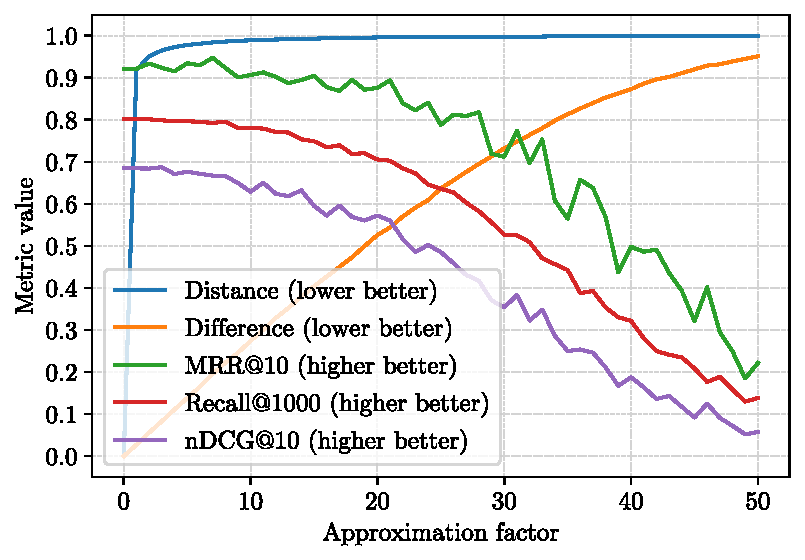
\includegraphics[width=1.0\textwidth]{knn-search-0-50} % chktex 8
	\caption{Search accuracy for $\beta \in \{ 0.0, \ldots, 50.0 \}$}\label{figure:knn-search-coarse}
\end{figure}


				We have run two sets of experiments to see how these metrics change with varying security parameter $\beta$.
				For first the set of $\beta$ values, we ranged the parameter from 0 to 50 with increment of $1.0$, see \cref{figure:knn-search-coarse}.
				Higher values of $\beta$ predictably degraded the search accuracy, but we wanted to see how quickly and after which values of $\beta$ the accuracy starts to fall noticeably.

				First, we notice that the result difference grows close to linearly with $\beta$, which means that each new security level knocks out a few correct responses from the set proportionally.
				Second, we see that the result distance jumps immediately to almost \SI{100}{\percent}, which means that even tiny approximation term significantly perturbs the order of the responses, but given low difference, not the content of the result.
				Finally, we observe that at about $\beta = 9$, the \acrshort{trec} metrics start to fall sharply and throughout the entire range of $\beta$ they fall in accord.

				For the maximum vector length of 11, the $\beta$ value that hides half of the input bits is $\beta = \sqrt{11} \approx 3.3$.
				To see the metrics behavior at around this point, we ran the experiments again, now ranging $\beta$ in finer manner, from $0.0$ to $5.0$ with the increment of $0.1$, see \cref{figure:knn-search-fine}.
				We confirm that for $\beta = \sqrt{\max N}$, the values of the ranking quality metrics are sufficiently close to the plaintext values.
				\emph{We therefore conclude that the bit-security \acrshort{dcpe} offers comes cheap in terms of search accuracy.}

				\begin{figure}[h]
	\centering
	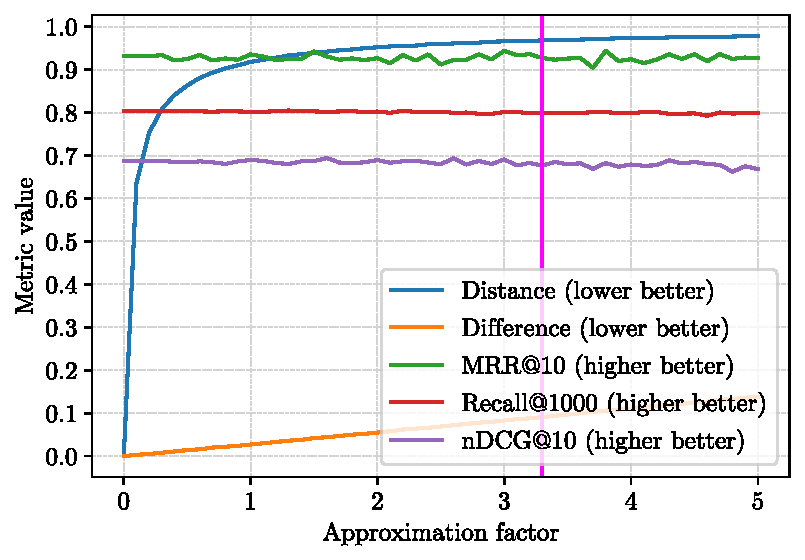
\includegraphics[width=1.0\textwidth]{knn-search-0-5}  % chktex 8
	\caption[Search accuracy for $\beta \in \{ 0.0, \ldots, 5.0 \}$]{
		Search accuracy for $\beta \in \{ 0.0, \ldots, 5.0 \}$.
		{\color{magenta}Highlighted} is $\beta = \sqrt{\max N}$ for $\max N \approx 11$ being the longest vector in the dataset.
	}\label{figure:knn-search-fine}
\end{figure}


	\section{Security against attacks}\label{section:knn-snapshot:attacks}

		The second part of a practical and secure outsourced similarity search application is the protection against attacks.
		In this set of experiments we adapt a recent \acrshort{ml}-based attack by \textcite{embedding-attacks}.
		\textcite{embedding-attacks} offer three attacks against the text embeddings:
		\begin{enumerate*}[label={(\roman*)}]
			\item \emph{the inversion attack}, which recovers a set of words from a document embedding,
			\item \emph{the attribute inference attack} that recovers some property of the document by its embedding, such as the gender or age of its author, and
			\item \emph{the membership inference attack}, which reveals whether a given document was or was not in the training set for the embedding model.
		\end{enumerate*}
		The inversion attack can be run in two modes, the white-box and the black-box.
		The white-box attack assumes the access to an embedding model and therefore can directly use its architecture and parameters to invert the inputs.
		The black-box attack relies only on being able to use the model to produce an embedding from a document, similar to how a generic embedding \acrshort{api} would work.
		We use this latter black-box inversion attack in our experiments since it most closely matches the adversary capabilities in our outsourced database setting.

		\subsection{Black-box model inversion attack \texorpdfstring{\cite{embedding-attacks}}{}}

			The black-box inversion attack assumes no knowledge of the embedding model, it can only use it to produce the embeddings.
			In this section we follow the original notation from \cite{embedding-attacks}.

			The attack works by training another model $\Upsilon$ to recognize the correlation between the set of words $\mathcal{W}(x)$ of a document $x$ and its embedding $\Phi(x)$.
			The attacker uses some auxillary dataset $\database_\text{aux}$ (same domain works predictably better than cross domain), and produces a collection of $ ( \Phi(x), \mathcal{W}(x) ) $ for all $x \in \database_\text{aux}$.
			The adversary then trains the attack model $\Upsilon$ to maximize $ \log \Pr_\Upsilon ( \mathcal{W}(x) | \Phi(x) ) $ over dataset $ ( \Phi(x), \mathcal{W}(x) ) $.
			Finally, the adversary simply queries the model with the embedding $ \Upsilon( \Phi( x ) ) $ and recovers the original words $\mathcal{W}(x)$.

			\textcite{embedding-attacks} offer two models for the inversion attack.
			The \acrfull{mlc} model assigns a binary label of whether a word is in the set for each word in the dictionary.
			The objective function is
			\[
				\mathcal{L}_{\text{\acrshort{mlc}}} = -\sum_{ w \in \mathcal{V} } \left[ y_w \log( \hat{y}_w ) + (1 - y_w) \log(1 - \hat{y}_w) \right]
			\]
			where
			\begin{itemize}
				\item $\mathcal{V}$ is a set of possible words, a dictionary,
				\item $\hat{y}_w = \Pr_\Upsilon( y_w | \Phi( x ) )$ is the predicted probability of word $w$ given $\Upsilon$ conditioned on $\Phi( x )$, and
				\item $y_w = 1$ if word $w$ is in $x$ and 0 otherwise.
			\end{itemize}

			A disadvantage of \acrshort{mlc} model is that it predicts all words independently.
			\textcite{embedding-attacks} therefore offer a more sophisticated approach based on \cite{msp}.
			A \acrfull{msp} recurrent neural network predicts the next word in the set conditioned on the embedding $\Phi( x )$ and the up-to-date predicted set of words.
			The objective function is
			\[
				\mathcal{L}_{\text{\acrshort{msp}}} = \sum_{ i = 1 }^\ell \frac{1}{| \mathcal{W}_i |} \sum_{w \in \mathcal{W}_i } - \log \Pr_\Upsilon( w | \mathcal{W}_{ < i }, \Phi( x ) )
			\]
			where $\mathcal{W}_{ < i }$ is the set of already predicted words up to a timestamp $i$ and $\mathcal{W}_i$ is the set of words left to predict.
			According to experiments in \cite{embedding-attacks}, \acrshort{msp} outperforms \acrshort{mlc}.

		\subsection{Experimental evaluation}\label{section:knn-snapshot:attacks:experiments}

			We have contacted the authors of \cite{embedding-attacks} and obtained a prototype code they used to run the attack.\footnote{
				\url{https://github.com/google/embedding-tests}
			}
			The model $\Upsilon$ is implemented as a one-layer \acrshort{lstm} with \num{300} hidden units.
			The model is trained for 30 epochs with Adam optimizer \cite{adam-optimizer}, learning rate of $10^{-3}$ and batch size of 256.
			The actual implementation uses TensorFlow \cite{tensorflow} (version 1) and is naturally optimized for \acrshort{gpu} training.

			We run two sets of experiments corresponding to two adversarial settings.
			First, similar to \cite{embedding-attacks}, we assume that the adversary has a black-box access to the embedding model $\Phi$ and can use it to train $\Upsilon$, and we call this experiment a \emph{public model}.
			This setting corresponds to a scenario when the system uses some open embedding model with little to no alterations (i.e., Google AI Platform Training\footnote{
				\url{https://cloud.google.com/ai-platform/training/docs/algorithms/bert}
			}).
			Second, we assume a more realistic scenario where the embedding model $\Phi$ is not available, and the adversary can only use the system as a whole.
			That is, for a given document $x$, the adversary can only produce the encrypted embedding $\algo{Enc}{\Phi(x)}$.
			We call this experiment a \emph{private model}.
			In both experiments the actual outsourced database is encrypted and the difference is in the dataset $\database_\text{aux}$ on which the adversary can train the attack model $\Upsilon$.
			In the public model experiment the adversary trains on plaintext embeddings while in the private model environment she trains on the already encrypted embeddings.

			For both experiments we have used two datasets.
			The first dataset is a BookCorpus \cite{bookcorpus} that \textcite{embedding-attacks} used.
			With this dataset we have been able to verify that our adapted attack implementation produces similar results to original \cite{embedding-attacks}.
			The second dataset is the \acrshort{trec} 2020, same as in \cref{section:knn-snapshot:search}.
			With this dataset we can link together the search accuracy and attack efficiency for the same levels of security.

			\subsubsection{Attack efficiency metrics}

				In line with \cite{embedding-attacks}, we define the attack efficiency metrics similar to a generic \acrshort{ml} measurers of accuracy --- precision, recall and \FOne{} score.
				Precision in our setting is defined as the number of words that the model predicted and that are part of an embedded sentence (i.e., true positives) over the total number of predicted words (all positives).
				Recall is defined as the number of correctly predicted words (true positives) over the number of all words in the sentence (true positives plus false negatives).
				\FOne{} score is then the harmonic mean of these two:
				\[
					\FOne = 2 \cdot \frac{ \mathsf{precision} \cdot \mathsf{recall} }{ \mathsf{precision} + \mathsf{recall} }
				\]

				We go a step further in this direction and given the context of the model --- recovering a set of words from a sentence embedding --- also track the fraction of common words (a.k.a., stop-words) in the predicted set.
				\acrshort{bert} explicitly encourages including the stop-words in the input because their relative position matters for the context and thus embedding.
				However, the attack only produces an unordered set of words and not their relative position.
				Therefore, the \emph{model prediction quality}, the \FOne{} score, may seem high, but it may not imply high \emph{attack efficiency}, because a huge fraction of predicted words are common and thus contribute little to added adversary knowledge.
				We define the list of stop words as pronouns, verb forms of ``be'', ``have'' and ``do'', some modal verbs, compound forms (e.g., ``you'll''), negations, articles, certain prepositions, conjunctions, adverbs and some more high-frequency words.\footnote{
					The list is adapted from the Snowball processing language: \url{http://snowball.tartarus.org/algorithms/english/stop.txt}.
				}
				We also include punctuation and digits in the list, as \acrshort{bert} tokenizes these along with the rest of the words.

			\subsubsection{Baselines}\label{section:knn-snapshot:attacks:experiments:baselines}

				\begin{figure}[h]
	\centering
	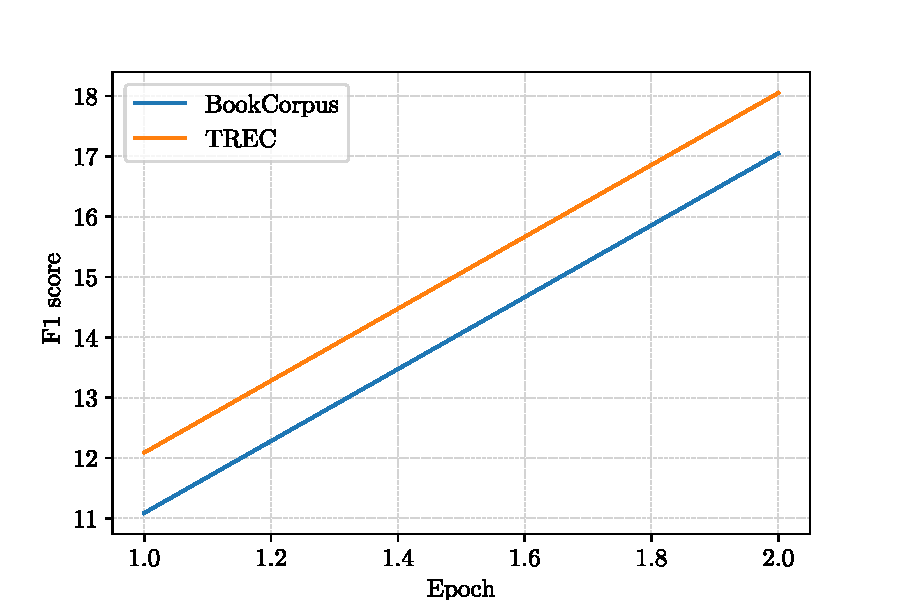
\includegraphics[width=1.0\textwidth]{knn-epochs} % chktex 8
	\caption[Inversion attack F1 score for different epochs]{
		Inversion attack F1 score for different epochs and for both datasets.
	}\label{figure:knn-epochs}
\end{figure}


				We have established two baselines between which the attack performance over encrypted inputs is assumed to lie.
				The first baseline is the attack on the plaintext inputs (referred to as \emph{plaintext attack}), a replica of the original attack from \cite{embedding-attacks}.
				The second baseline is the attack on the random embeddings (referred to as \emph{random attack}), which, counterintuitively, does not produce close to zero \FOne{} score.

				In both cases, we have trained the attack model for 30 epochs, see \FOne{} score on \cref{figure:knn-epochs}.
				We note a number of observations:
				\begin{enumerate*}[label={(\roman*)}]
					\item we have replicated the efficiency result of the black-box model inversion attack from \cite[Table 2, \FOne{} score, same domain, $\mathcal{L}_{\text{\acrshort{msp}}}$, \acrshort{bert}]{embedding-attacks},
					\item for the plaintext attack, the \FOne{} score stops growing after about $10_\text{th}$ epoch,
					\item the random attack produces a far-from-negligible \FOne{} score,
					\item \acrshort{trec} dataset is much less susceptible to the attack than the originally used BookCorpus.
				\end{enumerate*}

				On this latter observation, we speculate that the reason is in the size of the input document, and to the lesser extent different embedding mechanism.
				BookCorpus input document, as used in \cite{embedding-attacks}, is merely a sentence, while \acrshort{trec} document is a larger paragraph.
				We have tuned the maximum token sequence length (shorter sequences are padded, larger ones are truncated), but it yielded no improvement.
				From a purely combinatorial perspective, we conclude that the larger input looses more information while being embedded in the same-sized vector.

				The case of random attack is puzzling, as one would expect that there is no information to recover from an a-priori information-less (random) inputs.
				We have dived deeper than \FOne{} score and inspected the actual words that the attack recovered and observed that almost all of them are stop-words and punctuation.
				That is, the attack merely established that the input document contained a period, coma, ``the'' and ``a'', and it happened to be right some of the time.
				While such inversion technically results in an \FOne{} score as high as about \SI{22}{\percent}, it does not necessarily translate into an information leakage or a privacy violation.
				We therefore include an evaluation of recovered words as part of our larger analysis.

				We have run all experiments for both BookCorpus and \acrshort{trec} datasets, and we have noticed that although the absolute values of attack efficiency are higher for BookCorpus, all relations and correlations are the same for both datasets.
				We therefore report on the more relevant \acrshort{trec} dataset in the rest of the chapter.

			\subsubsection{Public model}

				For the public model setting we have used the trained model $\Upsilon$ from the baseline experiments and ran it against the encrypted embeddings.
				That is, for all documents $x$ in $\database_\text{aux}$, we recovered a set of words from the encrypted embeddings $\Upsilon( \algo{Enc}{ \Phi(x) } )$ and compared it to the set of words in the original document $\mathcal{W}(x)$.
				We have repeated the process for different values of $\beta \in \{ 1.0, \ldots, 50.0 \}$, see \cref{figure:knn-public}.

				\begin{figure}[h]
	\centering
	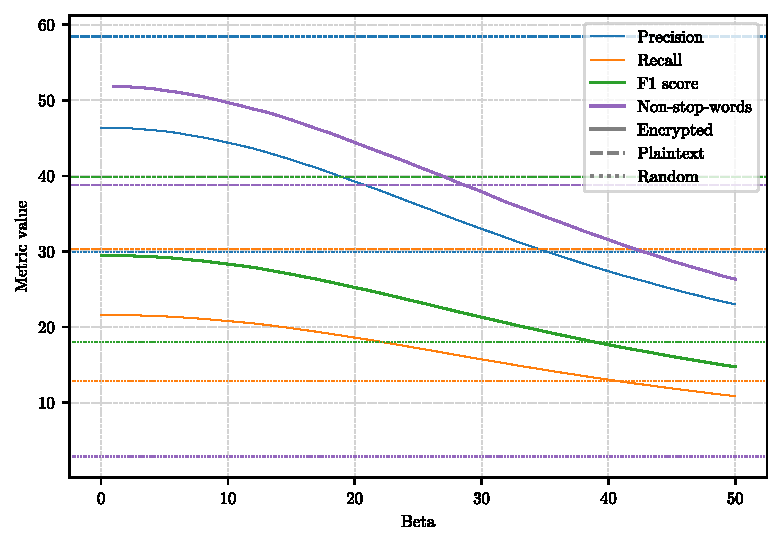
\includegraphics[width=1.0\textwidth]{knn-public} % chktex 8
	\caption[Inversion attack accuracy metrics for different $\beta$ for \acrshort{trec} dataset]{
		Inversion attack {\color{MatplotlibOne}precision}, {\color{MatplotlibTwo}recall}, {\color{MatplotlibThree}\FOne{} score} and {\color{MatplotlibFive}percentage of stop-words among recovered words} for plaintext attack (dashed), random attack (dotted) and different values of $\beta$ (solid) for the \acrshort{trec} dataset.
		Horizontal bars depict the baselines.
	}\label{figure:knn-public}
\end{figure}


				We observe that even for $\beta = 0$, the attack efficiency drops sharply compared to the plaintext baseline.
				We also see that the metric values drop further as $\beta$ increases, starting slowly for small $\beta$, then accelerating for $\beta$ 10 to 30 and then slowing down again.
				Interestingly, we observe that the attack efficiency dives below the lower baseline, the random embeddings.
				We conclude that $\beta \approx 27$, which is about 2.5 times the maximum length of the input vectors, produces the security equivalent to symmetric encryption.
				Finally, we note that the fraction of stop-words grows fast as the security increases.

			\subsubsection{Private model}

				For the private model experiments we have trained the model $\Upsilon$ on the already encrypted embeddings for 30 epochs.
				That is, the model $\Upsilon$ is trained on $ ( \algo{Enc}{ \Phi(x) }, \mathcal{W}(x) ) $ pairs from the training dataset and then we run predictions for the encrypted auxillary embeddings, similar to public model.
				The training and validation datasets are encrypted with the same set of public and private parameters (i.e., same key \key{}, $s$ and $\beta$).

				\begin{table}[!ht]
	\renewcommand{\arraystretch}{1.2}
	\sisetup{detect-all = true}
	\begin{tabular*}{\linewidth}{ !{\extracolsep\fill} l c c >{\bfseries}c c } % chktex 26
		\toprule
			Dataset (encrypted with $\beta$)	& Precision				& Recall				& \FOne{} score 		& Non-stop-words		\\
		\midrule
			$\beta = 0$							& \SI{41.59}{\percent}	& \SI{23.36}{\percent}	& \SI{29.91}{\percent}	& \SI{3.67}{\percent}	\\
			$\beta = \ceil{\sqrt{\max N}} = 4$	& \SI{41.91}{\percent}	& \SI{23.75}{\percent}	& \SI{30.32}{\percent}	& \SI{4.96}{\percent}	\\
			$\beta \approx \max N = 11$			& \SI{40.82}{\percent} 	& \SI{24.20}{\percent} 	& \SI{30.39}{\percent}	& \SI{5.18}{\percent}	\\
			$\beta \approx 2 \cdot \max N = 22$	& \SI{40.44}{\percent} 	& \SI{23.75}{\percent} 	& \SI{29.92}{\percent}	& \SI{5.76}{\percent}	\\
		\midrule
			Random embeddings					& \SI{35.91}{\percent}	& \SI{26.49}{\percent}	& \SI{30.49}{\percent}	& \SI{0}{\percent}		\\
		\bottomrule
	\end{tabular*}
	\sisetup{detect-none = true}
	\caption[Inversion attack performance for the private model experiments]{
		Black-box inversion attack performance for the private model experiments.
		The attack model $\Upsilon$ is both trained and validated on the specified datasets.
	}%
	\label{table:knn-private}
\end{table}


				We have chosen $\beta$ values of $0.0$ and $4.0$ as well as random embeddings to produce the datasets, see \cref{table:knn-private}.
				We immediately notice that the attack model accuracy metrics are similar among all three datasets, with $\beta = 4.0$ and random being almost equal.
				This result implies that for the case of private model --- when the adversary has only black-box access to the system as a whole --- the protection by the \acrshort{dcpe} is absolute.

	\section{Search accuracy against security tradeoff}

		Equipped with the empirical data from experiments on search accuracy and attack efficiency, we can correlate these values with the security parameter, the approximation term $\beta$.

		\begin{figure}[h]
	\centering
	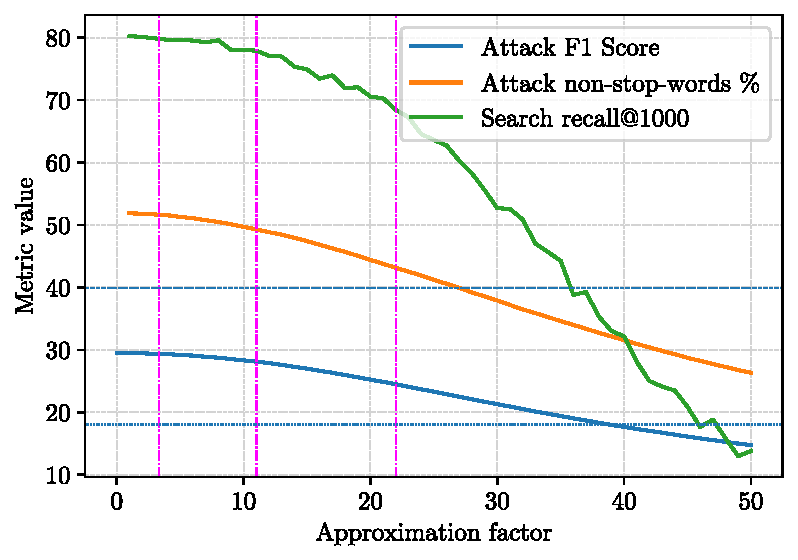
\includegraphics[width=1.0\textwidth]{knn-tradeoff} % chktex 8
	\caption[The correlation of search accuracy and the attack efficiency with $\beta$]{
		The correlation of search accuracy (the {\color{MatplotlibThree}recall@1000}) and the attack efficiency (the {\color{MatplotlibOne}\FOne{} score} and the {\color{MatplotlibTwo}percent of non-stop-words}) with the approximation term $\beta$.
		The {\color{magenta}vertical bars} show special values of $\beta$: $\sqrt{\max N}$, $\max N$ and $2 \cdot \max N$ for $\max N \approx 11$ being the longest vector in the dataset.
	}\label{figure:knn-tradeoff}
\end{figure}


		We note that the search accuracy degrades faster than attack efficiency, which implies that there is a tradeoff between functionality and security.
		Depending on the accuracy loss that the application can tolerate, the plot on \cref{figure:knn-tradeoff} can tell what level of protection against the inversion attack would be at that search accuracy.
		This plot also demonstrates the levels of accuracy and security for the $\beta$ as a derivative of the dataset, in particular, the length of the longest vector embedding $\max N$.

		We observe that at $\beta = \sqrt{\max N}$, the search accuracy corresponds to a plaintext dataset and the attack efficiency has dropped significantly compared to the plaintext version.
		We also see that at $\beta = \max N$ both search accuracy and attack efficiency drop insubstantially compared to $\beta = \sqrt{\max N}$.
		Finally, we note that at $\beta = 2 \cdot \max N$, although both measures drop significantly, after that point the accuracy goes down much faster, which implies that increasing $\beta$ beyond twice the longest vector size is pessimal.
		This value of $\beta$ is also close to a point where the attack \FOne{} score intercepts the \FOne{} score of a random embedding attack, which further confirms that this value of $\beta$ is optimal.

		\emph{Given the significant drop of attack efficiency for smaller $\beta$ while retaining almost optimal search accuracy, we conclude that our method of applying a \acrlong{dcpe} to an embedding to protect \acrshort{knn} queries is efficient.}
		The system we developed is also highly tuneable, with $\beta$ corresponding to the application-specific accuracy and security requirements.
		Finally, the construction is cheap in terms of performance and functionality --- the encryption of inputs is very fast and is done only once as a preprocessing step, and the existing algorithms work naturally over encrypted data.

		% TODO: axis 10pt, legend 8 pt.
		% TODO: fix manual constants in plots.

	\section{Conclusions}

		In this work we have developed and analyzed the mechanism of answering \acrshort{knn} queries securely in outsourced setting.
		We have adapted a \acrshort{dcpe} scheme, ran experiments on search accuracy and inversion attack efficiency over encrypted inputs.
		We have analyzed the correlation between the accuracy and security, and have concluded on viability and efficiency of the general approach.

		\subsubsection{Future Work}

			An immediate deeper analysis of inversion attack over encrypted embeddings may include an evaluation of the words that the attack model returns beyond simple matching against the set of stop-words.
			It is reasonable to assume that with stronger encryption the \emph{quality} of the predicted words may degrade, where the quality may be defined as the frequency of a word in the vocabulary, for example.

			Another direction can be running other attacks against the embedding, beyond the inversion attack.
			These may be some of the \textcite{embedding-attacks} attacks or adaptations of lots of general attacks against \acrshort{ml} models, like membership attacks \cite{membership-attacks,enhanced-membership-attacks}.

			Finally, the \acrshort{dcpe} adapted from \cite{dcpe} preserves Euclidean distance.
			It would be interesting to explore which results the inner-product distance comparison preserving encryption would produce.
